\documentclass{article}
\usepackage{german}
\usepackage[latin1]{inputenc}
\usepackage{a4wide}
\usepackage{epsfig}
\usepackage{amssymb}
\usepackage{fancyvrb}
\usepackage{alltt}


\title{NetBeans --- Kurzanleitung}
\author{Karl Stroetmann}

\begin{document}
\maketitle

Die Software \textsl{NetBeans} ist eine \textsl{Java} \textsc{IDE}.  Die Abk\"urzung
\textsc{IDE} steht f\"ur \emph{integrated development environment}, \textsl{NetBeans} ist
also eine komplette Entwicklungs-Umgebung f\"ur \textsl{Java}.  F\"ur den Anf\"anger ist der
Gebrauch einer solchen Entwicklungs-Umgebung nicht unbedingt empfehlenswert, da das
Erlernen der Bedienung einer solchen Umgebung mit erheblichem Zeitaufwand verbunden ist.
Am Anfang ist es besser, diese Zeit in das Erlernen der Programmiersprache \textsl{Java}
zu investieren.  Kein Programmierer kommt allerdings mittelfristig um die Verwendung eines
Debuggers herum.  
Ziel dieser Kurzanleitung ist es daher, Sie mit den wichtigsten Features des Debuggers
vertraut zu machen, der in \textsl{NetBeans} integriert ist.

\section{Start der Entwicklungs-Umgebung}
Im Übungsraum ist \textsl{NetBeans} unter dem Pfad \\[0.1cm]
\hspace*{1.3cm} \texttt{/opt/netbeans-4.1/bin/netbeans} \\[0.1cm]
abgelegt.  Am einfachsten ist es, wenn Sie am Ende der Datei \texttt{\symbol{126}/.bashrc}
die folgende Zeile einf\"ugen: \\[0.1cm]
\hspace*{1.3cm} \texttt{export PATH=/opt/netbeans-4.1/bin/:\symbol{36}PATH} \\[0.1cm]
Dann k\"onnen Sie die Entwicklungs-Umgebung mit dem Befehl \\[0.1cm]
\hspace*{1.3cm} \texttt{netbeans}\\[0.1cm]
starten.

\section{Laden eines Programmes}
Wie in der Einleitung schon erw\"ahnt macht es wenig Sinn, wenn Sie sich schon gleich zu
Anfang mit dem in \textsl{NetBeans} integrierten Editor auseinander setzen.  Es ist
einfacher, wenn Sie die \textsl{Java}-Programme zun\"achst weiter mit einem ihnen vertrauten
Editor wie \texttt{xemacs}, \texttt{emacs}, \texttt{kate} oder \texttt{vi} erstellen.  Dann m\"ussen Sie
aber wissen, wie Sie ein \textsl{Java}-Programm in die Entwicklungs-Umgebung laden k\"onnen.
Ich nehme im Folgenden an, dass Sie irgendwo ein Verzeichnis \texttt{Java-Examples} haben 
und dass Sie  diesem Verzeichnis f\"ur jedes Projekt, dass Sie bearbeiten, einen Unterordner
anlegen.  Konkret nehmen wir an, dass das Verzeichnis \texttt{Java-Examples} eine
Unterordner \texttt{Calculator} enth\"alt und dass sich in diesem Unterordner die
\textsl{Java}-Dateien befinden, deren Funktionalit\"at sie testen wollen.  
Konkret wollen wir annehmen, dass Sie dort die Dateien aus dem Tape-Archive
\\[0.1cm]
\hspace*{1.3cm}
\texttt{http://www.ba-stuttgart.de/\symbol{126}stroetma/Java/calculator.tar} \\[0.1cm]
installiert haben.  Es handelt sich hierbei um das in der Vorlesung besprochene Programm
zur Auswertung arithmetischer Ausdr\"ucke. Das Starten des Debuggers verl\"auft nun wie folgt:
\begin{enumerate}
\item Öffnen Sie eine  Shell und starten Sie \textsl{NetBeans} mit dem Kommando
      \texttt{netbeans}.  Falls das nicht funktioniert, m\"ussen Sie den vollen Pfad
      angeben: \\[0.1cm]
      \hspace*{1.3cm} \texttt{/opt/netbeans-4.1/bin/netbeans}
\item Öffnen Sie das Men\"u ``\texttt{\underline{F}ile} und w\"ahlen Sie dort den Eintrag
      ``\texttt{Ne\underline{w} Project}$\dots$''.
      Alternativ k\"onnen Sie auch die Taste \framebox{\texttt{Ctrl+Shift-N}} bet\"atigen.
\item Es erscheint nun ein Fenster, indem Sie unter der Überschrift
      \texttt{\underline{C}ategories}  die Kategorie des Projektes festlegen k\"onnen.
      Voreingestellt ist hier \texttt{General} und das ist f\"ur unsere Zwecke gerade richtig.

      Au{\ss}erdem k\"onnen Sie unter der Überschrift \texttt{\underline{P}rojects}
      die Art des Projektes festlegen.  Hier w\"ahlen Sie \\[0.1cm]
      \hspace*{1.3cm} \texttt{Java Project with Existing Sources} \\[0.1cm]
      und klicken anschlie{\ss}end auf den Button ``\texttt{Next>}''.
\item Es erscheint ein neues Fenster, in dem Sie zun\"achst einen Namen f\"ur das Projekt festlegen.
      Wir w\"ahlen den Namen ``\texttt{Calulator}''.
      Gleichzeitig k\"onnen Sie auf dieser Seite noch der Name eines Verzeichnisses angeben,
      in dem \textsl{NetBeans} Daten zu dem neuen Projekt ablegt. 
      Die Voreinstellung ist, dass der Projekt-Ordner in ihrem Home-Verzeichnis  
      abgelegt wird und den selben Namen hat wir das Projekt.  Da es nicht sehr sinnvoll
      ist, das Home-Verzeichnis mit solchen Projekt-Ordnern zuzum\"ullen, empfiehlt es sich,
      in dem Home-Verzeichnis einen Ordner ``\texttt{NetBeans-Projects}'' anzulegen und als
      Projekt-Ordner dann den Ordner ``\texttt{\symbol{126}/NetBeans-Projects/Calculator}''
      anzugeben.   Anschlie{\ss}end klicken Sie wieder auf den Button ``\texttt{Next>}''.
\item Nun erscheint ein Fenster, indem Sie das Verzeichnis angeben k\"onnen, indem sich die
      \textsl{Java}-Dateien befinden.  Bet\"atigen Sie hierzu die Schaltfl\"ache
      \texttt{\underline{A}dd Folder} neben dem Fenster mit dem Label
      \texttt{\underline{S}ource Package Folders}.
      Anschlie{\ss}end geben Sie das Verzeichnis \\[0.1cm]
      \hspace*{1.3cm} 
      ``\texttt{Java-Examples/Calculator}'' \\[0.1cm]
      an. Danach bet\"atigen Sie die
      Schaltfl\"ache \texttt{\underline{F}inish}.
\item Nun sind die \textsl{Java}-Dateien geladen und es erscheint ein Fenster,
      dessen linke obere Ecke die in Abbildung \ref{fig:left} gezeigte Form hat.
\begin{figure}[!h]
  \centering
   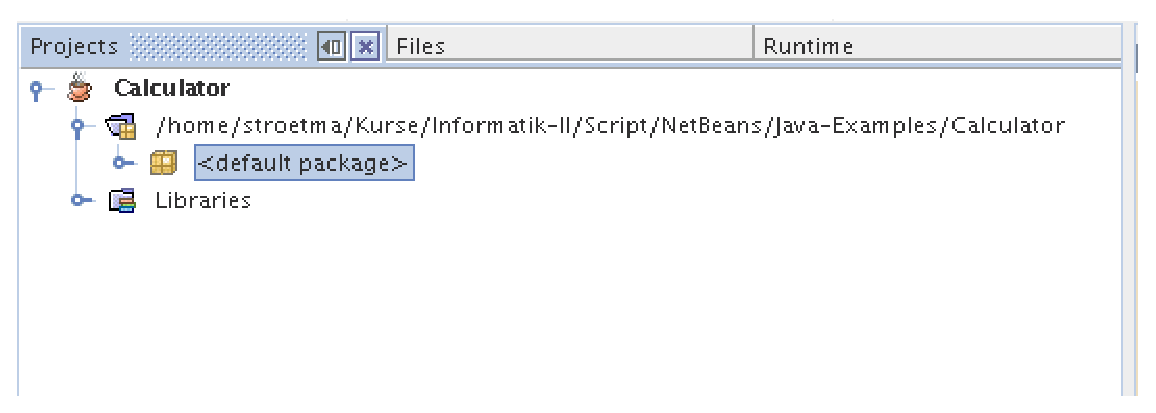
\epsfig{file=left,scale=0.7}
  \label{fig:left}
\end{figure}
      Klicken Sie auf den blauen Schalter links neben dem Text ``\texttt{<default package>}'',
      so werden die Namen der \textsl{Java}-Dateien angezeigt, die sich in dem Verzeichnis
      befinden.  Die Datei, die die Methode \texttt{main}() enth\"alt, ist durch ein kleines
      gr\"unes Dreieck markiert.
      Anschlie{\ss}end kann durch einen Doppel-Klick eine dieser Dateien ausgew\"ahlt werden.
      Wir w\"ahlen die Datei \texttt{Calulator.java} aus.  Diese Datei wird nun im rechten
      Teil des Debuggers angezeigt. 
\end{enumerate}

\section{Verwendung des Debuggers}
Bevor wir den Debugger laufen lassen, sollten wir Halte-Punkte (\emph{break points})
setzen.  Wir gehen dazu in die Zeile, in der wir den Haltepunkt setzen wollen.
In unserem Fall w\"ahlen wir in dem Konstruktor \texttt{Calulator} die Zeile mit der ersten
\texttt{while}-Schleife  und dr\"ucken 
\\[0.1cm]
\hspace*{1.3cm} \framebox{\texttt{Ctrl-F8}} \\[0.1cm]
Die Zeile, in der sich der Cursor befindet, wird dann rot unterlegt um anzuzeigen, dass
ein Haltepunkt gesetzt wurde.  Eine nochmalige Bet\"atigung der Taste
\framebox{\texttt{Ctrl-F8}} 
w\"urde den Haltepunkt wieder ausschalten.  Um nun den Debugger zu starten, bet\"atigen wir
die Taste \\[0.1cm]
\hspace*{1.3cm} \framebox{\texttt{F5}}. \\[0.1cm]
Es erscheint ein Fenster, indem wir nach der ``\emph{Main Class}'' gefragt werden.  
Das ist die Klasse, deren Methode \texttt{main}() wir laufen lassen wollen.
Wir w\"ahlen dort die Klasse \texttt{Calculator} aus.  Danach l\"auft der Debugger los.  Da das
Programm eine Eingabe (n\"amlich den arithmetischen Ausdruck, der berechnet werden soll)
erwartet, \"offnet sich in der linken unteren Ecke der \textsl{NetBeans}-Oberfl\"ache ein
Textfeld mit dem Label \texttt{\underline{I}nput}.  Nachdem wir dort den Text \\[0.1cm]
\hspace*{1.3cm} \texttt{1 + 2 * 3 - 4} \\[0.1cm]
eingegeben haben, schlie{\ss}en wir die Eingabe ab indem wir ein \framebox{\texttt{Return}} eingeben 
und anschlie{\ss}end  die rechts von diesem Text-Feld befindliche Schaltfl\"ache
\texttt{\underline{C}lose Input} bet\"atigen.   Das Programm l\"auft nun bis zu dem
Haltepunkt, den wir gerade gesetzt haben.
Wenn wir das Programm jetzt weiterlaufen lassen, dann  wollen wir sowohl die lokalen
Variablen als auch die Member-Variablen beobachten.  Dazu suchen wir zun\"achst im Editor die
Member-Variablen \texttt{mTokens}, \texttt{mArguments} und \texttt{mOperators}.  Wir
bewegen den Cursor an den Anfang der Variablen und setzen jeweils durch
dr\"ucken der Taste \\[0.1cm]
\hspace*{1.3cm} \texttt{Ctrl-Shift-F7} \\[0.1cm]
einen Beobachtungs-Punkt (\emph{watch point}).
Um das Fenster, das die Beobachtungs-Punkte anzeigt, sichtbar zu machen, w\"ahlen wir in dem
Men\"u \texttt{\underline{W}indow} den Eintrag
\texttt{De\underline{b}ugging}$\rightarrow$\texttt{\underline{W}atches} aus.  Alternativ
k\"onnen wir auch die Taste \\[0.1cm]
\hspace*{1.3cm} \texttt{Ctrl-Shift-2} \\[0.1cm]
bet\"atigen.  Da das Fenster mit den Beobachtungs-Punkten jetzt das Fenster mit den lokalen
Variablen verdeckt, schieben wir es \"uber das Fenster mit dem Titel 
``\texttt{Navigator - Calculator}'', dass sich mittig am linken Rand der
\textsl{NetBeans}-Oberfl\"ache befindet.  Das Fenster mit den Beobachtungs-Punkten enth\"alt
eine Tabelle, in der neben den Namen der Variablen noch die Typen und Werte angegeben
sind.  Weder die Typen noch die Werte sind f\"ur uns interessant, was wir sehen wollen ist
eine textuelle Darstellung der Variablen.  Dazu klicken wir auf die Schaltfl\"ache \"uber dem
Scroll-Bar am rechten Rand des Fensters mit dem Titel ``\texttt{Watches}''.  Es erscheint ein Fenster in dem wir
\texttt{toString()} ausw\"ahlen und \texttt{Type} and \texttt{Value} abw\"ahlen.
Dasselbe machen wir in dem Fenster, das die lokalen
Variablen anzeigt.  Dieses Fenster befindet sich rechts unten in der
\textsl{NetBeans}-Oberfl\"ache.

Jetzt k\"onnen wir mit dem eigentlichen Debuggen beginnen.  Hierzu k\"onnen wir die folgenden
Tasten verwenden:
\begin{enumerate}
\item \framebox{\texttt{F7}} f\"uhrt eine Zeile des Programms aus.
      Falls diese Zeile den Aufruf einer Methode enth\"alt, so springt
      die Kontrolle zu der Methode.
\item \framebox{\texttt{F8}} f\"uhrt ebenfalls eine Zeile des Programms aus.
      Im Unterschied zu \framebox{\texttt{F7}} springt \framebox{\texttt{F8}}
      aber \"uber den  Aufruf einer Methode hinweg, das hei{\ss}t dass ein Methoden-Aufruf in
      einem einzigen Schritt durchgef\"uhrt wird.
\item \framebox{\texttt{Alt-Shift-F7}} beendet die Abarbeitung der gerade abgearbeiteten
      Methode und springt zur aufrufenden Methode zur\"uck.
\item \framebox{\texttt{Ctrl-F5}}  l\"asst den Debugger bis zum n\"achsten Haltepunkt laufen.
\item \framebox{\texttt{Shift-F5}} stoppt den Debugger.
\end{enumerate}
Damit haben wir die wichtigsten zum Debuggen ben\"otigten Funktionalit\"aten vorgestellt.

\section{Der Editor}
Um Fehler, die beim Debuggen gefunden werden, schnell korrigieren zu k\"onnen ist es
sinnvoll, sich zumindest einen groben Überblick \"uber den Editor zu verschaffen.
 Der Editor unterscheidet sich nicht wesentlich von anderen Editoren.
Wir stellen die allerwichtigsten Funktionen des Editors vor:
\begin{enumerate}
\item Das Abspeichern einer Datei geschieht wie bei den meisten Editoren mit \framebox{\texttt{Ctrl-S}}.
\item \framebox{\texttt{Ctrl-F}} startet die Suche.
\item \framebox{\texttt{Ctrl-Z}} macht die letzte Änderung r\"uckg\"angig.
\item \framebox{\texttt{Ctrl-Leertaste}} startet die \textsl{Java}-Vervollst\"andigung.
      Diese ist ein sehr n\"utzliches Feature, dass wir jetzt n\"aher kennenlernen wollen.
      Wir gehen dazu an das Ende einer beliebigen Methode  und geben dort am Anfang einer
      neuen Zeile den Text ``\texttt{BigI}'' ein. Anschlie{\ss}end bet\"atigen wir
      die Taste \framebox{\texttt{Ctrl-Leertaste}}.  Nun vervollst\"andigt der Editor 
      den Text automatisch zu ``\texttt{BigInteger}''.  Wir deklarieren eine Variable
      \texttt{a}, schreiben in der  n\"achsten Zeile den Text ``\texttt{a.}'' und dr\"ucken
      wieder \framebox{\texttt{Ctrl-Leertaste}}. Dann erscheint \"uber dem Cursor ein neues
      Fenster, in dem s\"amtliche Methoden der Klasse \texttt{BigInteger} aufgelistet sind.
      Mit den Tasten ``$\downarrow$'' und ``$\uparrow$'' k\"onnen wir hier die verschiedenen Methoden
      aktivieren.  Es wird die Dokumentation der gerade aktivierten Methode angezeigt.  Haben wir
      die gew\"unschte Methode gefunden, so k\"onnen wir Sie mit \framebox{\textsl{Return}}
      ausw\"ahlen.

      Sollte uns das Fenster mit den Methoden aus irgendeinem Grunde st\"oren, so k\"onnen wir
      es durch Bet\"atigen des \framebox{\texttt{Escape}}-Taste schlie{\ss}en.
\item \framebox{\texttt{Ctrl-K}} und \framebox{\texttt{Ctrl-L}} aktiviert das sogenannte
      \emph{Word Matching}.  Nehmen Sie an, dass Sie irgendwo oberhalb der Stelle, an der
      Sie gerade editieren, das Wort \\[0.1cm]
      \hspace*{1.3cm} ``\texttt{mDonauDampfschiffFahrtsGesellschaft}'' \\[0.1cm]
      im Text stehen haben.  Jetzt wollen Sie dieses Wort wieder eingeben.
      Dann reicht es  aus, die ersten paar Buchstaben (beispielsweise ``\texttt{mDo}'')
      dieses Wortes einzugeben und anschlie{\ss}end die Taste \framebox{\texttt{Ctrl-K}} oder
      \framebox{\texttt{Ctrl-L}} zu bet\"atigen.   Die Taste \framebox{\texttt{Ctrl-K}} sucht dann r\"uckw\"arts im
      Text nach einem Wort, dass mit dem Text ``\texttt{mDo}'' anf\"angt und vervollst\"andigt
      den bisher eingegebenen Text entsprechend.  Analog sucht die Taste \framebox{\texttt{Ctrl-L}}
      vorw\"arts im Text.  Gibt es mehrere W\"orter, die mit dem Text ``\texttt{mDo}''
      anfangen, so k\"onnen diese der Reihe nach durch nochmaliges Dr\"ucken der Tasten 
      \framebox{\texttt{Ctrl-K}} oder \framebox{\texttt{Ctrl-L}} ausgew\"ahlt werden.
\item Schlie{\ss}lich sind in dem \textsl{NetBeans}-Editor eine Reihe Abk\"urzungen integriert.
      Wollen Sie beispielsweise den Text \\[0.1cm]
      \hspace*{1.3cm} \texttt{public static final String}\\[0.1cm]
      eingeben, so reicht es aus, den Text ``\texttt{psfs}'' einzugeben und anschlie{\ss}end
      die Leertaste zu bet\"atigen.  Dann wird der Text ``\texttt{psfs}'' entsprechend
      expandiert.  Sollten Sie tats\"achlich einmal den Text ``\texttt{psfs }'' w\"ortlich
      eingeben wollen, so m\"ussen Sie anstelle der Leertaste die Taste
      \framebox{\texttt{Shift-Leertaste}} bet\"atigen.

      Sie k\"onnen sich jederzeit die Liste der Abk\"urzungen ansehen, indem Sie 
      die Taste \framebox{\texttt{Alt-H}}+\framebox{\texttt{K}} bet\"atigen.
      Dann wird eine PDF-Datei angezeigt. Auf der ersten Seite finden Sie die
      Keyboard-Shortcuts, auf der zweiten Seite sind die Abk\"urzungen aufgelistet. 
\end{enumerate}

\end{document}
